\chapter{Method}
% describe method
% prerequisites: generative models. AE, VAE, GAN

% INTRO FIGURE: PART REPRESENTATION
% \begin{figure}[t]
	% \begin{subfigure}{0.3\linewidth}
	% \centering
	% \includegraphics[trim={0cm 0cm 0cm 0cm},clip, width=1.\linewidth]{fig/rep1_hq}\caption{}
	% \end{subfigure}
	% \begin{subfigure}{0.3\linewidth}
	% \centering
	% \includegraphics[trim={0cm 0cm 0cm 0cm},clip, width=1.\linewidth]{fig/rep2}\caption{}
	% \end{subfigure}
	% \begin{subfigure}{0.3\linewidth}
	% \centering
	% \includegraphics[trim={0cm 0cm 0cm 0cm},clip, width=1.\linewidth]{fig/rep3}\caption{}
	% \end{subfigure}
	% \caption{An object is represented in parts. Each part has a distinct spatial extend (part shape) and a corresponding feature descriptor (part appearance). (a) input image, (b) model output of part shapes (each plotted in a different color), (c) schematic illustration of part appearances}
	% \label{fig:representation}
% \end{figure}
%
	\begin{quotation}
		\textit{disentangle as many factors as possible, discarding as little information about the data as is practical} - Y. Bengio, A. Courville and P. Vincent \cite{bengio}
	\end{quotation}
	To capture an object in an abstract representation, we follow two key ideas: \emph{(i)} disassembling the object into its constituent parts and \emph{(ii)} disentangling spatial geometry (shape) from visual features (appearance). Hence, we model an object as a composition of parts, each part with a part appearance and a part shape, see Fig. \ref{fig:representation}. The part shape should correspond to the area in the image where the part is located, whereas the part appearance is a feature descriptor for that area. The overall object representation is then the collection of part shapes and part appearances. \\
	% \begin{equation}
	%(a, s) = \cup_i (f_i, p_i)
	%\end{equation}
	%\label{eq:representation}
	% enforcing locality of parts is important
	% what do our representations entangle still?:
	% shape: position, shape, size
	% appearance: illumination, color, texture, material
	\todo{local features theme}
	The disentanglement of shape and appearance can be enforced by demanding that shape is invariant under the transformation of appearance and vice versa. This is realized in a two-stream auto-encoding formulation. Here, an image is reconstructed from a combination of shape and appearance, with shape extracted from the appearance-transformed image and appearance from a shape-transformed image. Additionally, the part shape is tied to the location of the part in the image: an equivariance loss encourages that the part shape moves in unison with the part in the image. We implement these objectives into a loss framework, which is explained in sec. \ref{sec:framework}. \\
	To assert a decomposition into independent local parts, we ensure their local modelling and treatment throughout the whole pipeline. This is highlighted when describing the architecture in sec. \ref{sec:architecture}.

\section{Framework}\label{sec:framework}
	% CROSSING TASK FRAMEWORK
	\begin{figure}[t]
		\centering
		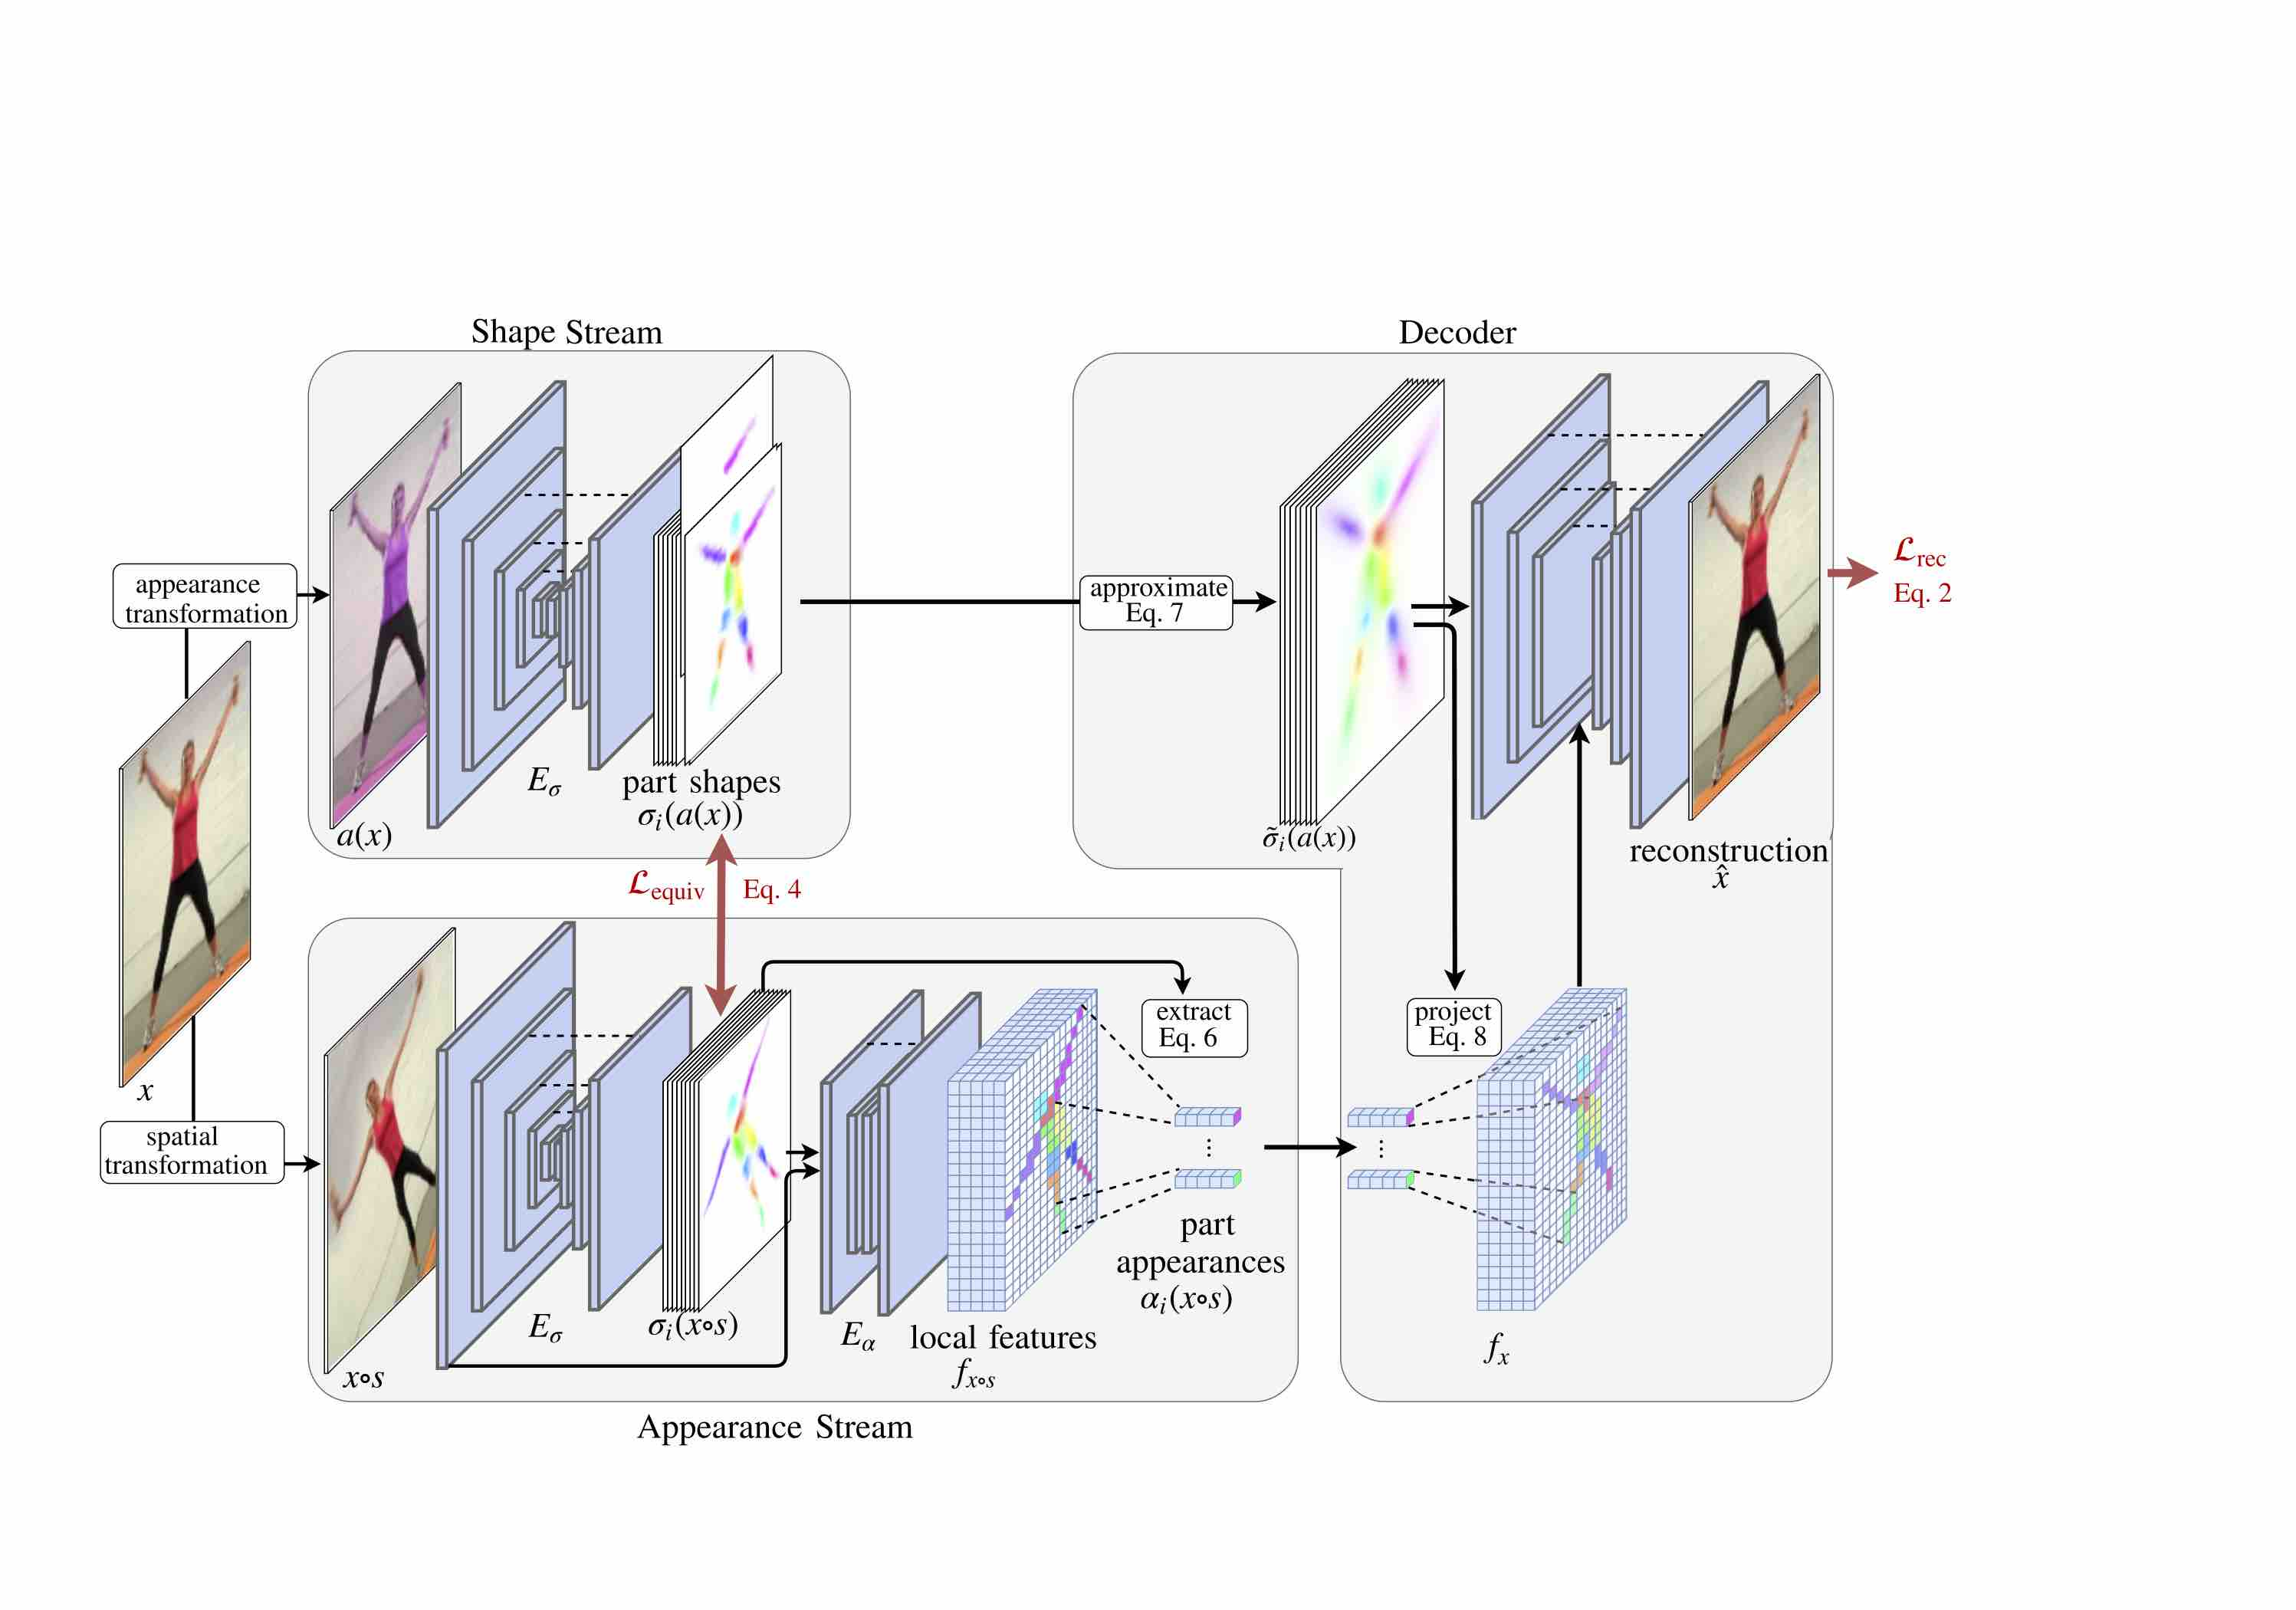
\includegraphics[trim={0cm 0cm 0cm 0cm},clip, width=1.\linewidth]{fig/architecture_final}
		\caption{Encoder $E$ encodes shape and appearance for two images $\pi(X)$ and $\phi(X)$, after recombination $R$ of $(f_{\pi(X)}, p_{\phi(X)})$ into latent image $Z$, the decoder $D$ reconstructs the image $X$.}
		\label{fig:framework}
	\end{figure}
	%Definitions
	We want to represent an object in an image $X$. Let us denote the part shape with $p_X$ and the part appearance with $f_X$. For an object with $n$ parts, the overall shape is constituted by the collection of its part shapes $p_X =  (p^1_X, ...,  p^n_X)$, the same goes for the appearance $f_X =  (f^1_X, ...,  f^n_X)$. We model the part appearances as feature vectors, the part shapes are chosen to be scalar fields like the image itself. Thereby one can establish a direct correspondence of locations in the image to locations in the shape representation.\todo{say the following or not?}\\
	%In contrast to other works, where object pose is often modeled by single points as landmarks, a representation based on a scalar field is much richer: whereas a landmarks inform about the exact position, the field-like representation also describes the size and shape of the object parts (see Fig.\ref{fig:representation}).
	% Transformations -> Crossing framework
	How do we disentangle the shape and appearance components in the representation? In general, a variation in shape will not affect appearance and vice versa. Thus, if we deliberately change shape without changing appearance, we can enforce the invariance of the appearance representation under such a change.
	We refer to these changes as shape transformations $\pi$, which, if applied to an image $X$, directly act on the underlying pixel space $\Lambda$.
	Along the same lines we can define appearance transformations $\phi$, which act on the image itself.
	The shape should be invariant under change of appearance, conversely, the appearance should be invariant under change of shape.
	In addition, the shape should transform in the same manner as the image.
	That means the shape representation is assumed to be equivariant under shape transformations.
	In summary:
	\begin{align}
		f_{\pi(X)}  &= f_{X} \tag{invariance of appearance}\\
		p_{\phi(X)} &= p_X  \tag{invariance of shape}\\
		p_{\pi(X)} &= \pi(p_X) \tag{equivariance of shape}
	\label{eq:invar}
	\end{align} % quad \forall i \leq n
	Our method builds on the auto-encoding paradigm, with part shapes and part appearances assuming the role of the latent code.
	To incorporate these constraints into the loss of an auto-encoder, we reconstruct an image $X$ not from the shape and appearance $(f_X, p_X)$ determined from the original image $X$, but from appropriately transformed images $(f_{\pi(X)}, p_{\phi(X)})$.
	If the invariance constraints, as formulated above, are fullfilled, these transformations do not change the latent code.
	Thus, the loss implicitly enforces invariance.
	To obtain shape and appearance, we encode both $\phi(X)$ and $\pi(X)$ with an encoder $\mathrm{E}$.
	And, after a recombination $\mathrm{R}$ (for details see sec. \ref{sec:architecture}) to a latent image $Z$, a decoder $\mathrm{D}$ reconstructs the image.
	This configuration is depicted in Fig. \ref{fig:framework}, the reconstruction loss $\mathcal{L}_{\textrm{rec}}$ is as follows:
	%\begin{align}
	%\mathcal{L}_{\textrm{rec}} &=  \lVert X -  \mathrm{D}[\mathrm{R}[\mathrm{E}(X)]]\rVert \\
	%&= \lVert  X  - \mathrm{D}[\mathrm{R}[ (f_X, p_X)]]\rVert \nonumber \\
	%&= \lVert  X  - \mathrm{D}[\mathrm{R}[ (f_{X_{\pi'}}, p_{X_{\phi'}}]]\rVert \nonumber
	%\end{align}
	%The to-be-reconstructed image $X_{\phi, \pi}$ has been subject to shape and appearance transformations $X \rightarrow \phi \circ \pi (X)$.
	%We instantiate this loss in a two-stream configuration, as shown in Fig. \ref{fig:framework}. %Encoder and decoder are the same for each stream, but image representations are crossed.
	%For simplicity we abbreviate $f = f_{\pi(X)}$, $f' = f_{\phi(X)}$ , $s = p_{\phi(X)}$ and $s' = p_{\pi (X)}$.
	%In accordance with the desired invariances, one can apply a transformation $\phi$ to the image, in order to selectively destroy appearance information in the shape representation and vice versa destroy shape information in the appearance representation with $\pi$.
	%The first stream encodes $\pi(X)$ to obtain $(a, s')$  and the second stream encodes $\phi(X)$ to obtain $(a', s)$.
	%Then appearance and shape representations are crossed.
	%After recombining $(a, s)$ to a feature volume $V$ (explained in detail in sec. \ref{sec:architecture}), the decoder reconstructs $X$.
	\begin{equation}
	\mathcal{L}_{\textrm{rec}}= \lVert  X  - \mathrm{D}[\mathrm{R}(f_{\pi(X)}, p_{\phi(X)})]\rVert
	\end{equation}
	\label{eq:loss_rec}
	%From an information perspective, we apply an appearance transformation to the image, to selectively destroy appearance information in the shape representation and vice versa destroy shape information in the appearance representation with a shape transformation.
	Let us examine what this formulation means on the level of a single part: the part appearance $f^i_X$ is extracted at locations in the spatially transformed image $p^i_{\pi(X)}$, but then used for reconstruction at the location in the original image $p^i_{X}$. For example in Fig.  \ref{fig:framework} the appearance of the arm will be extracted in a raised position, but then these features are used for reconstructing an arm in a lowered position. For this to succeed, firstly, the appearance features need to be sufficiently abstract. Secondly, part locations of the two images have to refer to the same part and track the location of it consistently. This part assignment consistency is an implicit way to improve equivariance under the shape transformations.\\
	%The shape also need to be invariant under appearance transformations, so part assignment needs to be consistent .
	%For video data the crossing task can be run on images pairs that show the same object in a different articulation (i.e. different frames of the video), enforcing equivariance of $s$ with respect to natural shape transformations. \\
	For a known shape transformation the equivariance of shape can also be encouraged explicitly with a loss. This has been used before in the context of unsupervised landmark learning by \cite{thewlis17, Zhang18} as a point-wise loss on a part probability map, encouraging the exact location of a part to transform accordingly. In our case, the part shapes shall not encode probability, but instead the spatial extend of a part. In approximation, we want the first two moments ($\mu, \Sigma$) to transform correctly. Thereby the extend and orientation of the parts is penalized in addition to the mere position.
	\begin{equation}
	\mathcal{L}_{\textrm{equiv}}^i = \mathcal{L}_{\mu}^i+ \mathcal{L}_{\Sigma}^i
	\label{covariance}
	\end{equation}
	The overall loss objective is the sum of the reconstruction loss and the equivariance loss for all $n$ parts:
	\begin{equation}
	\mathcal{L} = \sum_{i=1}^n \mathcal{L}_{\text{equiv}}^i + \mathcal{L}_{\textrm{rec}}
	\end{equation}


\section{Architecture}\label{sec:architecture}
	The auto-encoding pipeline consists of three stages, namely: \textbf{encoding} both shape and appearance for each part,  \textbf{recombining} this information meaningfully into a latent image and \textbf{decoding} this latent image to reconstruct the image. The whole process is sketched in Fig. \ref{fig:framework}, the operations in more detail are visualized in Fig. \ref{fig:x1}, \ref{fig:x2}, \ref{fig:x3},  \ref{fig:x4}. Throughout the procedure we maintain the local correspondence between the representation and the image: We ensure a local appearance extraction in the encoding, a local synthesis in the recombining and a local usage of the latent image in the decoding. These architectural restrictions enable a disentangled part representation with the interpretation of a part as a localized entity. \\

	\subsection{Analysis}
		${(f, p | X)}$\footnote{ For a slim notation, we leave out the explicit reference to the generic input image $X$ in this section: $f, p, f^i, p^i$ refer to $f_X, p_X, f^i_X, p^i_X$.} The encoding of shape and appearance given an image proceeds in two steps: \\
		\emph{(i.)} $(p|X)$: The part shapes are predicted given the image. To extract part shapes we use an hourglass\footnote{ We utilize hourglass neural network models in both steps, as these models are able to preserve pixel-wise locality, but integrate information from multiple scales \cite{hourglass}.}  neural network: The input is an image $X$, the output a stack of $n$ part shapes $s =  \{p^i| i=1, ...,  n\}$.\\ \emph{(ii.)} $(p|f,X)$: The part appearances $f =  \{f^i| i=1, ...,  n\}$ are predicted given the image and the part shapes. Again we use an hourglass network, albeit shallower. The input is the original image concatenated with the stack of part shapes. The output is a feature stack $F$. A part appearance is obtained by averaging the feature stack with the a part shape: $f^i = \sum_{x \in \Lambda} A(x) \frac{p^i(x)}{\sum_{x' \in \Lambda}p^i(x')} $. Each $f^i$ now describes the appearance of a part spatially localized by the part shape $p^i$. \\

	\subsection{Recombination of Factors}
		In the analysis-by-synthesis regime, once the object representation is successfully factorized, one can make assumptions on how the factors reunite to generate an image, following the knowledge and intuition about how objects give rise to images in the physical world.
		Firstly, we remerge shape and appearance into images of descriptors at the correct locations. For each part, appearance is multiplied with the corresponding shape, yielding $n$ part feature images: $z^i(x) = p^i(x) \cdot f^i$.
		Secondly, we reassemble the object from its parts: the part feature images $z^i$ are summarized by summing in a single image: $ Z(x) = \sum_i \frac{z^i(x)}{1 + \sum_j z^j(x)}$. The result is an image of part feature descriptors located according to their corresponding part shape, which we call latent image $Z$.\\


	\subsection{Synthesis}
		Finally, the latent image needs to be decoded to an image. This is done by a neural network decoder. The decoder architecture is modeled after the upsampling stream of a standard U-Net \cite{}. The latent image is scaled to different scales \todo{alter figure z1 etc} and inserted, after each layer, in addition to the part shapes \todo{why add shapes?}. As before, the crucial property of the parts that needs to be conserved is their local direct correspondence to the image. On the one hand, one needs to assure, that the receptive field of the neurons does not extend to the full image, in order to thwart a complex non-local interaction of part information. This is why we use only half of a U-Net instead of a complete U-Net or an hourglass architecture.
		On the other hand, it is essential to regularize the information already before passing it to the decoder. Keeping in mind that the part shape should be of rather simple geometry, we introduce a differentiable information bottlenecks, in order to prevent the shape from being scattered over the object. It is an approximation of the part shape as $\hat p^i(x) = \frac{1}{1 + (x -\mu)^T \Sigma^{-1} (x - \mu)}$, where $\mu$ and $\Sigma$ are the mean and the covariance matrix of the part shape $p^i$. This allows to pass second-order information such as size and orientation of the part to the decoder. Note that this operation are fully differentiable.


	\section{Implementation Details}\label{implementationdetails}
		The image resolution is $128 \times 128$, but the resolution of corresponding part shapes is $ 64 \times 64$. \\
		For the reconstruction  loss $\mathcal{L}_\text{rec}$ we use the $L_1$ or $L_2$ distance. To prevent parts from trying to explain the whole image, instead of focusing on the object, we also restrict the reconstruction loss to an area around the part shape: a sum of Gaussian approximations around the means of the part shapes is folded with the loss.\\
		In the decoder, the latent image Z is not only rescaled, but also filled with parts incrementally. At the lowest scale only some parts are inserted, with each scale parts are added until at the highest scale all parts are used. This makes the part decoding a hierarchical process. The underlying assumption is the parts exist at multiple scales.
		For landmark learning, we approximate the part shapes in the decoder in the bottleneck also with $\hat p^i(x) = \frac{1}{1 + (x -\mu)^T \Sigma^{-1} (x - \mu)}$, but fix the covariance $\Sigma$ to the identity matrix. Hence, effectively only information about the mean of each part shape can reach the decoder. This mean information is used as a landmark, so encouraging an accurate estimation of the mean through reconstruction is wanted.\todo{this needs further explanation or is dangerous}\\
		To instantiate shape transformations $\pi$, one needs image pairs that show the same object in a different articulation or position: For static images an artificial thin-plate spline transform (TPS) can be applied, which generalizes rotation, scaling, translation. For video data adjacent frames exhibit natural shape transformations. The appearance transformation $\phi$ is encompassing a colour augmentation, contrast variations, and changes in brightness. In general, the more selective the transformation distinguishes shape and appearance, the more invariant the representation.
